\section{Выполнение}

\subsection{Фрагмент кода}

Фрагмент кода представлен в листинге \ref{lst:fragment}.

\begin{lstlisting}[label=lst:fragment,caption=Фрагмент кода.]
	#include <pthread.h>
	#include <stdio.h>

	int var1 = 3, var2 = 2;
	int res1 = 0;

	void* thread1(void* arg) {
		var1++;
		var2++;
	}

	void* thread2(void* arg) {
		res1 = var1 + var2;
	}

	int main() {
		pthread_t t1, t2;
		pthread_create(&t1, NULL, thread1, NULL);
		pthread_create(&t2, NULL, thread2, NULL);

		pthread_join(t1, NULL);
		pthread_join(t2, NULL);

		printf("res1: %d\n", res1);

		return 0;
	}
\end{lstlisting}

\subsection{Описание модели}

Описание модели программы из листинга \ref{lst:fragment} представлено в листинге \ref{lst:model}.

\begin{lstlisting}[label=lst:model,caption=Описание модели.]
	short var1 = 3;
	short var2 = 2;
	short res1 = 0;

	proctype Thread1() {
		var1++;
		var2++;
	}

	proctype Thread2() {
		res1 = var1 + var2;
	}

	init {
		run Thread1();
		run Thread2();

		printf("Result: res1 = %d\n", res1)
	}
\end{lstlisting}

\subsection{Множества состояний}

Каждое состояние системы представляет собой тройку, описывающую значения переменных \textit{var1}, \textit{var2} и \textit{res1}. Таким образом, в представленной системе могут иметь место значения (для удобства наименования \texit{Thread1} и \texit{Thread2} приводятся как T1 и T2):

\begin{itemize}
	\item 3, 2, 0 -- начальное состояние системы;
	\item 3, 2, 5 -- T2 выполнил инструкцию, Т1 не начал выполнение;
	\item 4, 2, 5 -- T2 выполнил инструкцию, Т1 выполнил одну инструкцию;
	\item 4, 3, 5 -- T2 выполнил инструкцию, Т1 выполнил две инструкции;
	\item 4, 2, 0 -- Т1 выполнил инструкцию, Т2 не начал выполнение;
	\item 4, 2, 6 -- Т1 выполнил инструкцию, Т2 выполнил инструкцию;
	\item 4, 3, 6 -- Т1 выполнил инструкцию, Т2 выполнил инструкцию, Т1 выполнил инструкцию;
	\item 4, 3, 0 -- Т1 выполнил две инструкции, Т2 не начал выполнение;
	\item 4, 3, 7 -- Т1 выполнил две инструкции, Т2 выполнил инструкцию;
\end{itemize}

\subsection{Граф переходов между состояниями модели}

Граф переходов между состояниями модели представлен на рисунке \ref{img:trans}.

\begin{figure}[H]
	\centering
	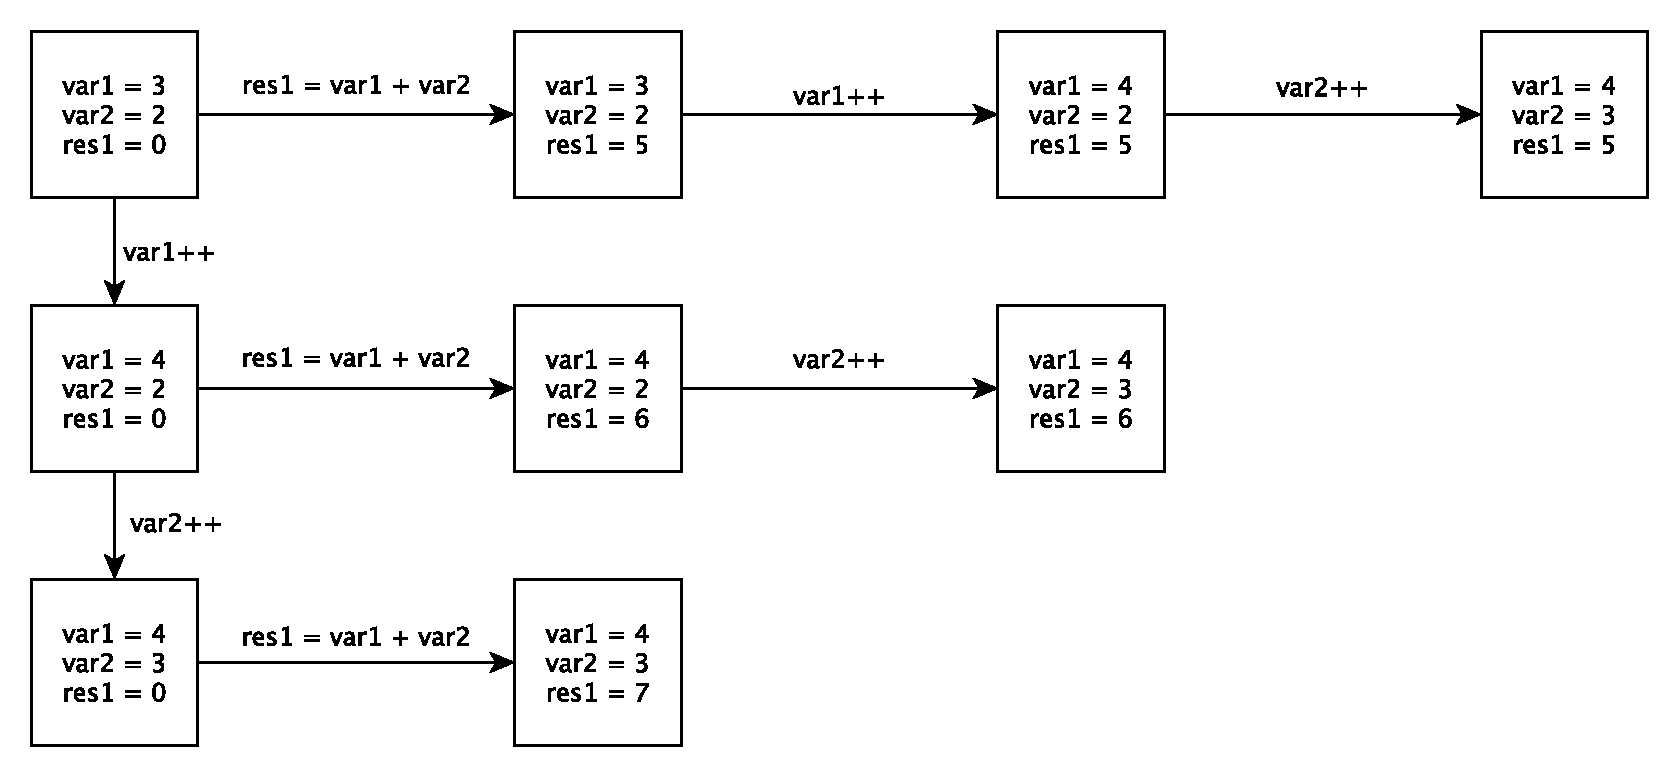
\includegraphics[width=\textwidth]{inc/trans.pdf}
	\caption{ Граф переходов между состояниями модели. }
	\label{img:trans}
\end{figure}

\pagebreak